\documentclass[11pt,a4paper]{article}
\usepackage[T1]{fontenc}
\usepackage[utf8]{inputenc}
\usepackage[english]{babel}
\usepackage{lmodern,amsmath,booktabs,graphicx}
\usepackage[margin=23mm]{geometry}
\usepackage{microtype}
\usepackage[hidelinks]{hyperref}
\graphicspath{{figures/}}
\title{Nooelec UWB Surveyor: apparent distance offset\\Measurement details and complex $S_{11}$ data}
\author{Technical note for John}
\date{9 October 2026}
\begin{document}
\maketitle
\noindent Dear John,\\[4pt]
Thank you for your help. This note documents the instrument, time-domain
processing and measurement geometry, and accompanies complex $S_{11}$ files
for a target-free background and three plate positions.
The purpose is to distinguish a common electrical delay from the change in
free-space distance, without assuming that the antenna alone explains the offset.

\section{Equipment and geometry}
\begin{itemize}
\item Instrument: LiteVNA 64, operated via USB using custom Python scripts.
\item Antenna: Nooelec UWB Surveyor, planar biconical PCB antenna,
$120\times120$ mm, marked v1.0b2 and 2025-10-15.
\item Target: an aluminum plate, parallel to the antenna PCB. Distances are
measured from the antenna's front surface to the plate and are approximate.
\item \textbf{Plate width, height and thickness: not yet supplied.}
\item The apparatus is used indoors on a table, with wooden supports and
nearby fixtures. No anechoic environment or multipath suppression is claimed.
\end{itemize}
The transparent panel visible in a previously shared setup photograph was
absent during the aluminum-plate measurements.
\begin{figure}[!ht]
\centering
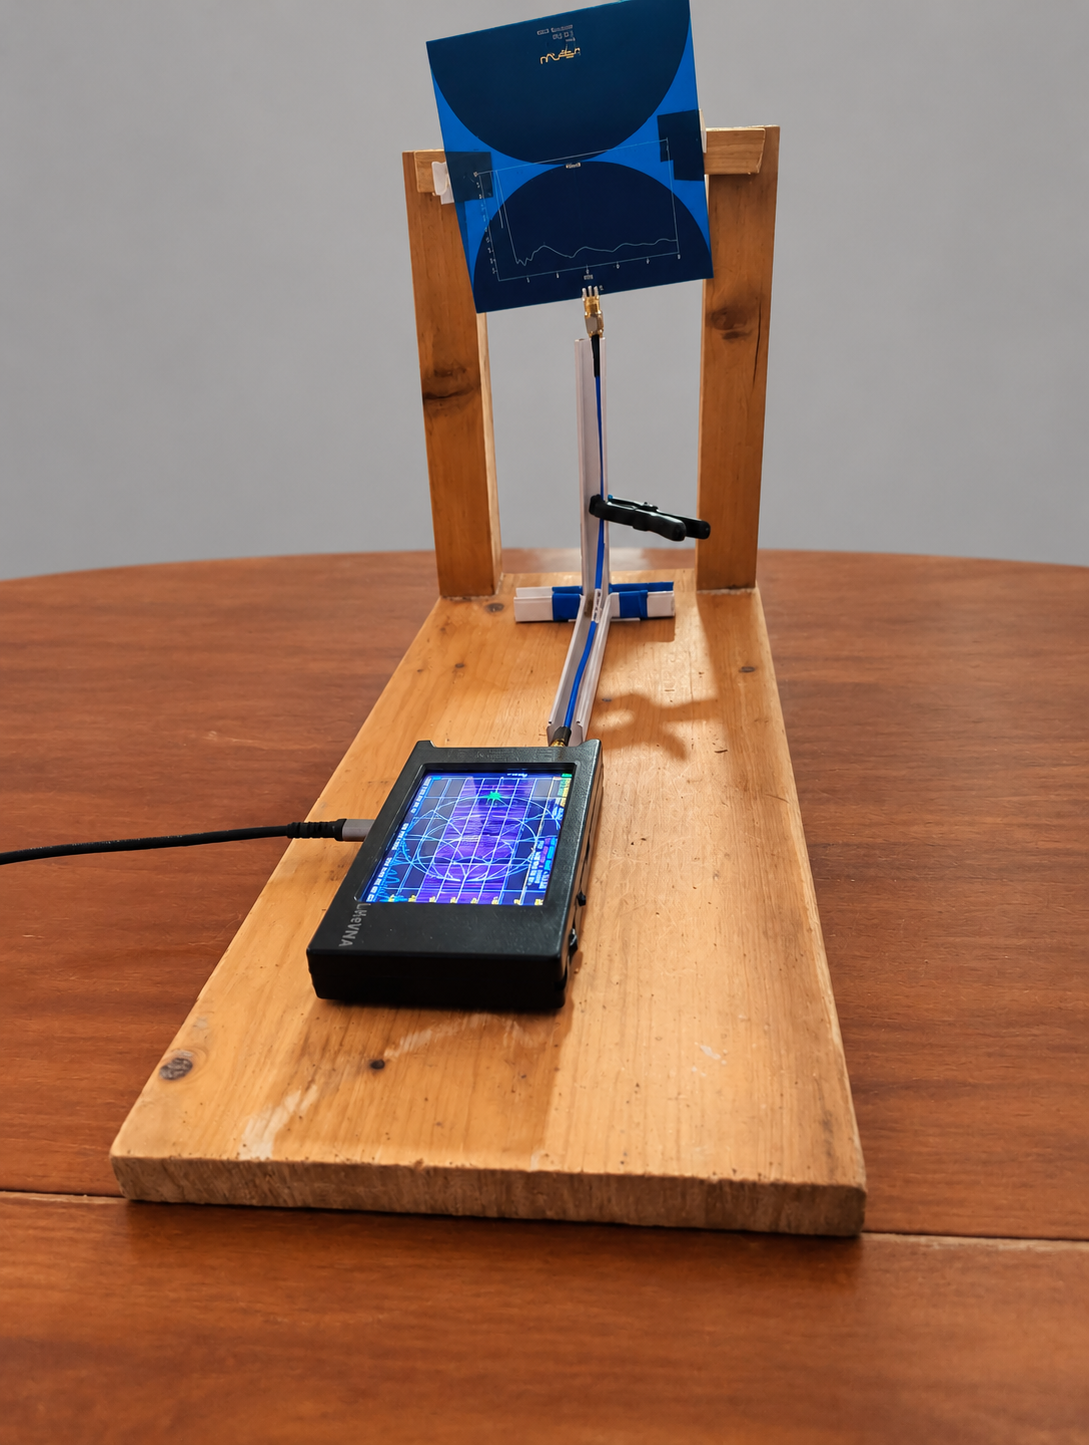
\includegraphics[height=5.4cm]{setup_edited.png}
\caption{Antenna, support, cable routing and VNA. This is an AI-retouched
presentation image: household surroundings and a person were removed.
It is not evidence of an uncluttered measurement environment or a dimensional
reference. The plate is not shown.}
\end{figure}

\clearpage
\section{Acquisition and processing}
\begin{center}
\begin{tabular}{ll}
\toprule
Frequency band & 1--6 GHz\\
Frequency samples & 201, uniformly spaced\\
Frequency step & 25 MHz\\
Plate averaging & 10 sweeps, complex arithmetic mean\\
Calibration & Software one-port SOL at the cable end\\
Window & Symmetric Hann, $w_k=\tfrac12[1-\cos(2\pi k/(N-1))]$\\
IFFT length & $16N=3216$ (zero-padding factor 16)\\
Reference impedance & $50\,\Omega$\\
\bottomrule
\end{tabular}
\end{center}
The firmware is read in raw mode, and the saved SOL coefficients are applied
in Python. The antenna is connected after the calibration plane; its radiating
transfer function is not de-embedded. The exported complex values have not been
windowed or background-subtracted.

For each plate position, the displayed method-A profile uses
\begin{align}
 R_k &= \overline{S}_{11,\mathrm{plate}}(f_k)
        -\overline{S}_{11,\mathrm{background}}(f_k),\\
 P_m &=16\left|\operatorname{IFFT}_{3216}(w_k R_k)_m\right|,\\
 d_m &=\frac{c}{2}\frac{m}{3216\,\Delta f},\qquad c=299792458\ \mathrm{m/s}.
\end{align}
The reported level is $20\log_{10}P_m$. The Hann coherent gain is not
normalized out. The frequency start contributes a phase factor to the complex
time response but does not change its magnitude envelope. The plotted
positive-distance interval is approximately 0--3 m.
The interpolated distance spacing is 1.86 mm; this is \emph{not} the physical
resolution. The bandwidth scale $c/(2B)$ is about 3 cm, and Hann broadens the lobes.

\section{Data supplied: 9 October 2026}
The currently available blue-antenna dataset contains three positions at
approximately 50, 60 and 70 cm. All three files have exactly the same frequency
grid, background and SOL coefficients; these were checked numerically.
The mapping between filenames and distances is recorded in the project's
existing comparison manifest.
\begin{center}
\begin{tabular}{lll}
\toprule
Measurement & UTC acquisition timestamp & Export basename\\
\midrule
Background & 15:26:25 & \texttt{background}\\
Plate, 50 cm & 15:27:14 & \texttt{plate\_50cm}\\
Plate, 60 cm & 15:27:44 & \texttt{plate\_60cm}\\
Plate, 70 cm & 15:27:56 & \texttt{plate\_70cm}\\
Independent SHORT & 10:09:10 & \texttt{independent\_short}\\
\bottomrule
\end{tabular}
\end{center}
Each basename is provided as CSV and Touchstone \texttt{.s1p} in \texttt{data/}.
CSV columns are frequency in Hz, real $S_{11}$, imaginary $S_{11}$.
Touchstone files use \texttt{\# Hz S RI R 50}. These are calibrated complex
means \emph{before} background subtraction. The SHORT uses the same SOL
coefficients but was acquired earlier in the day.

\clearpage
\section{Plate-position comparison}
\begin{figure}[htbp]
\centering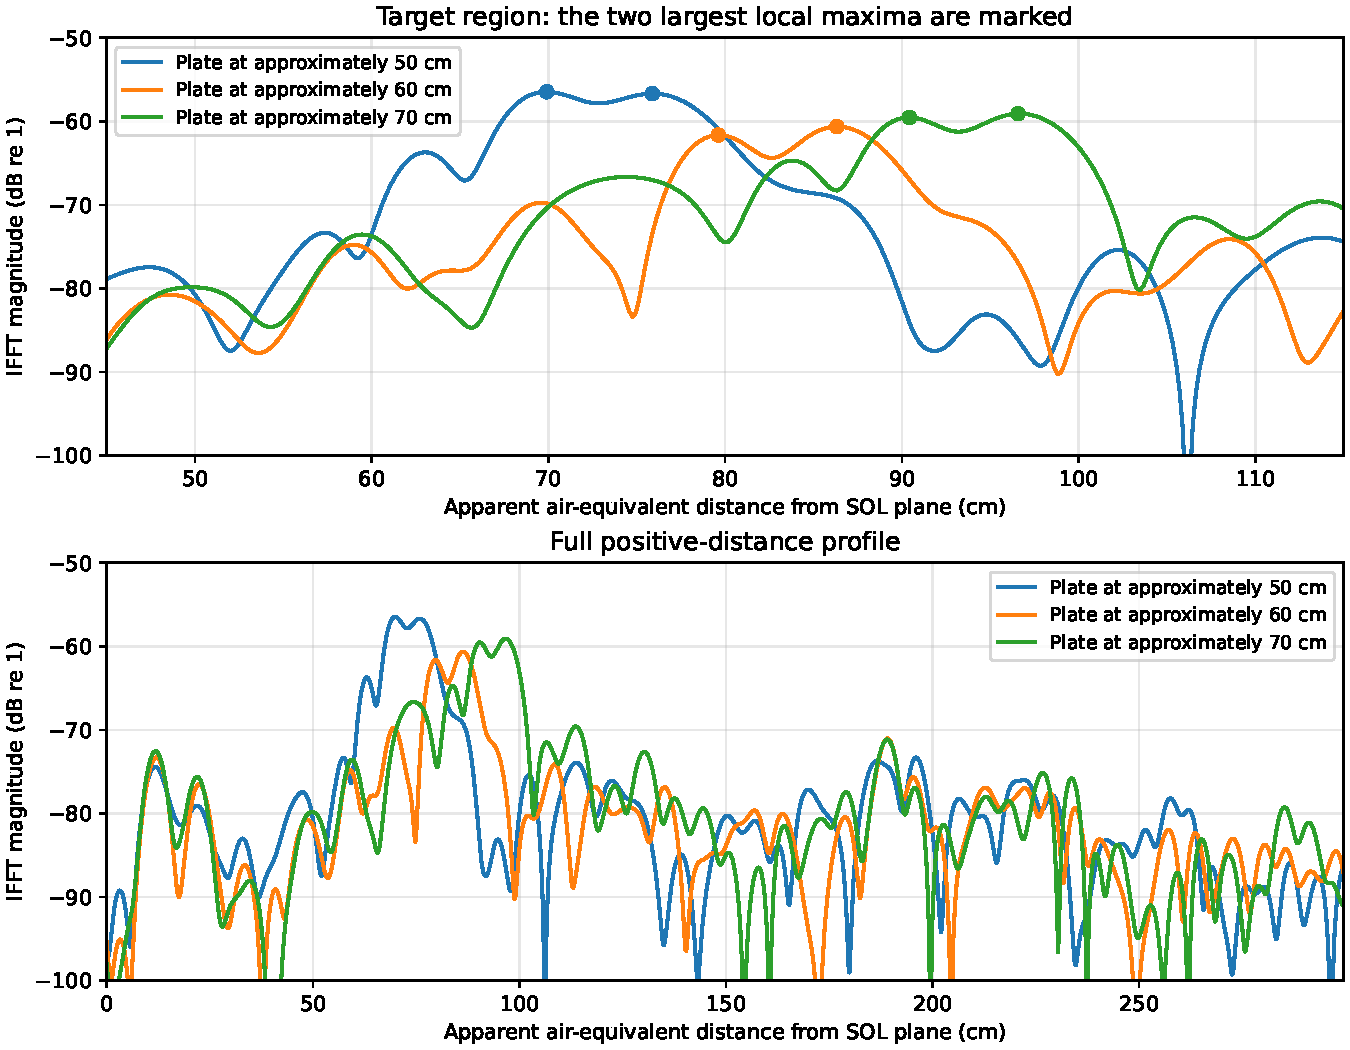
\includegraphics[width=\linewidth]{profiles.pdf}
\caption{9 October measurements processed with identical background subtraction,
Hann window and IFFT settings. No distance-offset correction or per-curve
amplitude normalization has been applied. The dots mark the two strongest
local maxima in each profile, without assigning them to physical interfaces.}
\end{figure}
\begin{center}
\begin{tabular}{rrrrr}
\toprule
Plate (cm)&Near peak (cm)&Far peak (cm)&Near offset (cm)&Far offset (cm)\\
\midrule
50&69.91&75.88&19.91&25.88\\
60&79.61&86.32&19.61&26.32\\
70&90.42&96.57&20.42&26.57\\
\bottomrule
\end{tabular}
\end{center}
The near-peak shifts are 9.69 and 10.81 cm for nominal 10 cm movements;
the far-peak shifts are 10.44 and 10.25 cm. The mean offsets are approximately
20.0 cm and 26.3 cm for the near and far branches, respectively.
The strongest peak changes branch between 50 and 60 cm, so simply selecting
the global maximum introduces a jump unrelated to the nominal displacement.
The paired peaks do not establish two physical target surfaces.

\clearpage
\section{Common echo-phase slope and deviations}
\begin{figure}[!ht]
\centering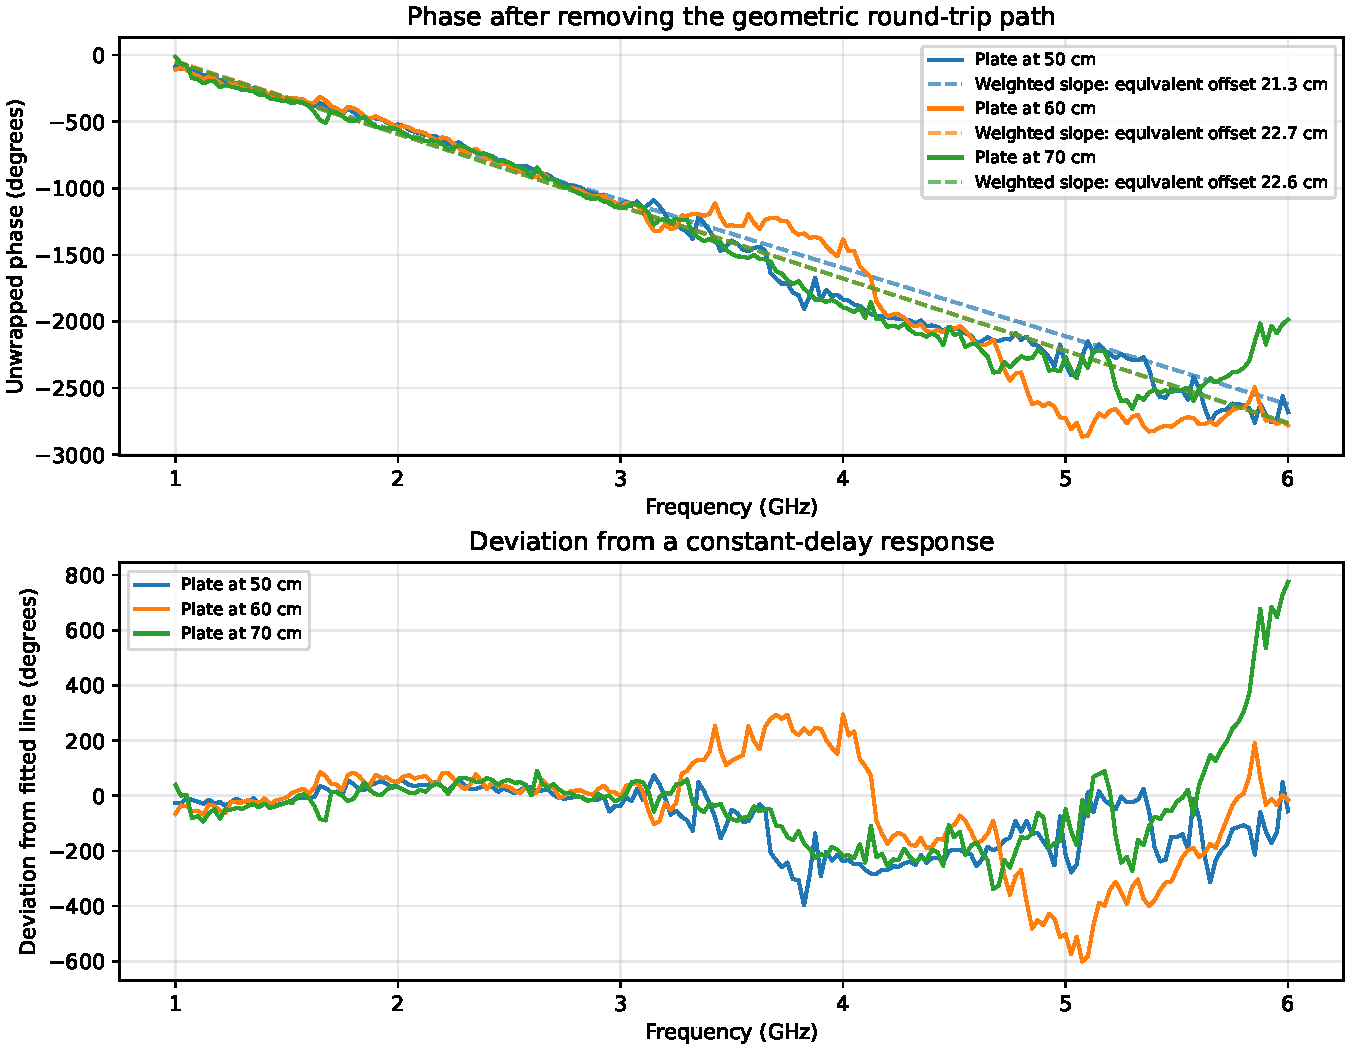
\includegraphics[width=\linewidth]{echo_phase.pdf}
\caption{English reproduction of the middle and bottom panels of
\texttt{phase\_echo\_bleue\_50\_60\_70cm.png}. Top: phase after removing
the nominal geometric round-trip path, with independent power-weighted
linear fits. Bottom: deviation from each fitted line. These are plate-minus-background
echoes measured with the blue antenna, not the antenna-only $S_{11}$.}
\end{figure}
The processing order is important: first remove the nominal free-space phase
from the complex echo, then unwrap its phase:
\[
H_d(f)=\bigl[\overline S_{11,d}(f)-\overline S_{11,\mathrm{bg}}(f)\bigr]
 e^{+\mathrm{j}4\pi f d/c},\qquad
\phi_d(f)=\operatorname{unwrap}\arg H_d(f).
\]
Each straight line is fitted over 1--6 GHz with weights proportional to
$|H_d(f)|^2$ and a free intercept. Its slope $b$ corresponds to
$\tau=-b/(2\pi)$ and an equivalent offset $c\tau/2$.
The offsets are approximately \textbf{21.3, 22.7 and 22.6 cm} for the
50, 60 and 70 cm positions. Their similar slopes support a common delay
component after nominal free-space propagation has been removed.

The lower panel shows departures from a constant-delay response, particularly
above approximately 3 GHz, where the echo magnitude also decreases.
These departures can include antenna dispersion, target/fixture multipath,
noise and phase-unwrapping errors near spectral minima. Weighting reduces
the influence of low-amplitude samples but cannot repair an unwrapping error.
The common slope alone does not uniquely identify the antenna radiation delay.

\clearpage
\section{Earlier observations, kept separate}
On 22 September, four approximate positions of 50, 60, 70 and 80 cm gave
near peaks of 68.4, 81.3, 91.7 and 100.9 cm, respectively, corresponding to
an average near-peak offset of about 20.6 cm. Those values are retained from
the earlier analysis in our correspondence. The original September acquisition
files are no longer present in the current workspace, so they are \emph{not}
the data exported with this note. The October dataset above independently
shows a similar near-peak offset.
An earlier experiment with a different, green antenna reportedly showed an
offset of approximately 38 cm. Its raw data and complete configuration are not
included, so it is not used here as a controlled antenna comparison.

\clearpage
\section{Independent SHORT check and questions}
\begin{figure}[htbp]
\centering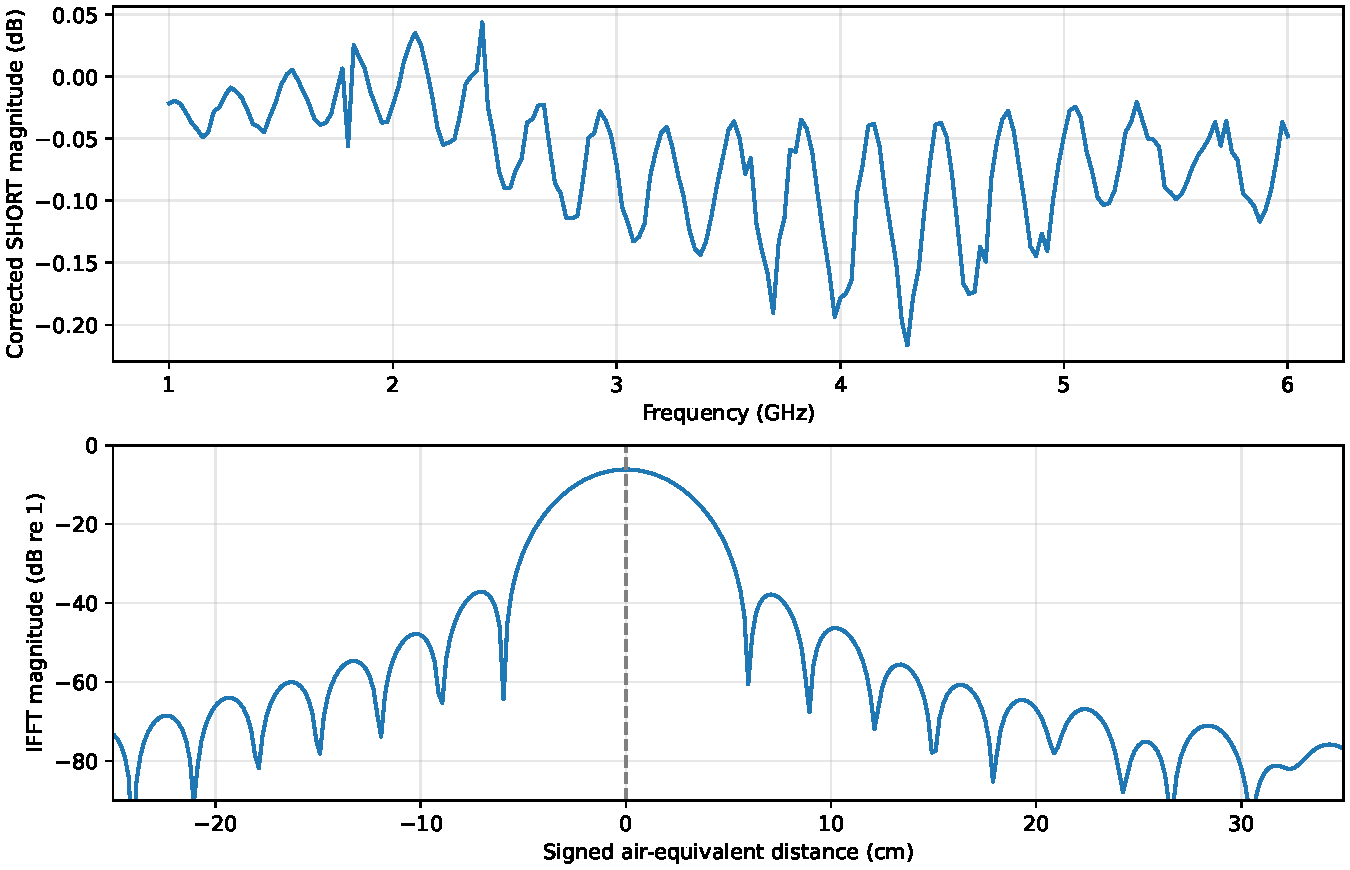
\includegraphics[width=\linewidth]{short.pdf}
\caption{A new SHORT acquisition on 9 October, corrected with the existing
SOL rather than used to fit it. The signed distance axis shows both sides of
zero. The SHORT profile is computed directly, without background subtraction.}
\end{figure}
This check tests the calibrated chain at the cable end. It does not measure
the antenna's radiation delay and does not rule out later drift, reconnecting
effects or room multipath. Its zero-distance response supports investigating
contributions introduced after the calibration plane.

A 21 cm apparent offset corresponds to a total round-trip delay of about
1.4 ns. We have not established a physical decomposition of that delay.
Could you advise on the following points?
\begin{enumerate}
\item Are group-delay or complex radiation-response data available for the
UWB Surveyor v1.0b2 over 1--6 GHz, referenced to the SMA connector?
\item Is its phase-center location versus frequency and observation direction
characterized, and what reference convention is used?
\item Could the feed structure and radiating response account for the common
near-peak offset, or for the paired-lobe profile? What measurement would best
distinguish these effects from fixture or room reflections?
\end{enumerate}
\noindent Manufacturer reference:
\href{https://www.nooelec.com/store/downloads/dl/file/id/110/product/339/uwb_surveyor_datasheet_revision_1.pdf}{UWB Surveyor datasheet, revision 1 (2022)}.
The published sheet does not specify group delay or phase-center coordinates;
it predates the marking on this antenna.
\end{document}
